\documentclass[11pt,]{article}
\usepackage{lmodern}
\usepackage{amssymb,amsmath}
\usepackage{ifxetex,ifluatex}
\usepackage{fixltx2e} % provides \textsubscript
\ifnum 0\ifxetex 1\fi\ifluatex 1\fi=0 % if pdftex
  \usepackage[T1]{fontenc}
  \usepackage[utf8]{inputenc}
\else % if luatex or xelatex
  \ifxetex
    \usepackage{mathspec}
  \else
    \usepackage{fontspec}
  \fi
  \defaultfontfeatures{Ligatures=TeX,Scale=MatchLowercase}
\fi
% use upquote if available, for straight quotes in verbatim environments
\IfFileExists{upquote.sty}{\usepackage{upquote}}{}
% use microtype if available
\IfFileExists{microtype.sty}{%
\usepackage{microtype}
\UseMicrotypeSet[protrusion]{basicmath} % disable protrusion for tt fonts
}{}
\usepackage[margin=4cm]{geometry}
\usepackage{hyperref}
\hypersetup{unicode=true,
            pdftitle={Exploratory data analysis and graphics (lab 2)},
            pdfauthor={2005 Ben Bolker, modified at several places by Bob Douma 2018},
            pdfborder={0 0 0},
            breaklinks=true}
\urlstyle{same}  % don't use monospace font for urls
\usepackage{color}
\usepackage{fancyvrb}
\newcommand{\VerbBar}{|}
\newcommand{\VERB}{\Verb[commandchars=\\\{\}]}
\DefineVerbatimEnvironment{Highlighting}{Verbatim}{commandchars=\\\{\}}
% Add ',fontsize=\small' for more characters per line
\usepackage{framed}
\definecolor{shadecolor}{RGB}{248,248,248}
\newenvironment{Shaded}{\begin{snugshade}}{\end{snugshade}}
\newcommand{\KeywordTok}[1]{\textcolor[rgb]{0.13,0.29,0.53}{\textbf{#1}}}
\newcommand{\DataTypeTok}[1]{\textcolor[rgb]{0.13,0.29,0.53}{#1}}
\newcommand{\DecValTok}[1]{\textcolor[rgb]{0.00,0.00,0.81}{#1}}
\newcommand{\BaseNTok}[1]{\textcolor[rgb]{0.00,0.00,0.81}{#1}}
\newcommand{\FloatTok}[1]{\textcolor[rgb]{0.00,0.00,0.81}{#1}}
\newcommand{\ConstantTok}[1]{\textcolor[rgb]{0.00,0.00,0.00}{#1}}
\newcommand{\CharTok}[1]{\textcolor[rgb]{0.31,0.60,0.02}{#1}}
\newcommand{\SpecialCharTok}[1]{\textcolor[rgb]{0.00,0.00,0.00}{#1}}
\newcommand{\StringTok}[1]{\textcolor[rgb]{0.31,0.60,0.02}{#1}}
\newcommand{\VerbatimStringTok}[1]{\textcolor[rgb]{0.31,0.60,0.02}{#1}}
\newcommand{\SpecialStringTok}[1]{\textcolor[rgb]{0.31,0.60,0.02}{#1}}
\newcommand{\ImportTok}[1]{#1}
\newcommand{\CommentTok}[1]{\textcolor[rgb]{0.56,0.35,0.01}{\textit{#1}}}
\newcommand{\DocumentationTok}[1]{\textcolor[rgb]{0.56,0.35,0.01}{\textbf{\textit{#1}}}}
\newcommand{\AnnotationTok}[1]{\textcolor[rgb]{0.56,0.35,0.01}{\textbf{\textit{#1}}}}
\newcommand{\CommentVarTok}[1]{\textcolor[rgb]{0.56,0.35,0.01}{\textbf{\textit{#1}}}}
\newcommand{\OtherTok}[1]{\textcolor[rgb]{0.56,0.35,0.01}{#1}}
\newcommand{\FunctionTok}[1]{\textcolor[rgb]{0.00,0.00,0.00}{#1}}
\newcommand{\VariableTok}[1]{\textcolor[rgb]{0.00,0.00,0.00}{#1}}
\newcommand{\ControlFlowTok}[1]{\textcolor[rgb]{0.13,0.29,0.53}{\textbf{#1}}}
\newcommand{\OperatorTok}[1]{\textcolor[rgb]{0.81,0.36,0.00}{\textbf{#1}}}
\newcommand{\BuiltInTok}[1]{#1}
\newcommand{\ExtensionTok}[1]{#1}
\newcommand{\PreprocessorTok}[1]{\textcolor[rgb]{0.56,0.35,0.01}{\textit{#1}}}
\newcommand{\AttributeTok}[1]{\textcolor[rgb]{0.77,0.63,0.00}{#1}}
\newcommand{\RegionMarkerTok}[1]{#1}
\newcommand{\InformationTok}[1]{\textcolor[rgb]{0.56,0.35,0.01}{\textbf{\textit{#1}}}}
\newcommand{\WarningTok}[1]{\textcolor[rgb]{0.56,0.35,0.01}{\textbf{\textit{#1}}}}
\newcommand{\AlertTok}[1]{\textcolor[rgb]{0.94,0.16,0.16}{#1}}
\newcommand{\ErrorTok}[1]{\textcolor[rgb]{0.64,0.00,0.00}{\textbf{#1}}}
\newcommand{\NormalTok}[1]{#1}
\usepackage{graphicx,grffile}
\makeatletter
\def\maxwidth{\ifdim\Gin@nat@width>\linewidth\linewidth\else\Gin@nat@width\fi}
\def\maxheight{\ifdim\Gin@nat@height>\textheight\textheight\else\Gin@nat@height\fi}
\makeatother
% Scale images if necessary, so that they will not overflow the page
% margins by default, and it is still possible to overwrite the defaults
% using explicit options in \includegraphics[width, height, ...]{}
\setkeys{Gin}{width=\maxwidth,height=\maxheight,keepaspectratio}
\IfFileExists{parskip.sty}{%
\usepackage{parskip}
}{% else
\setlength{\parindent}{0pt}
\setlength{\parskip}{6pt plus 2pt minus 1pt}
}
\setlength{\emergencystretch}{3em}  % prevent overfull lines
\providecommand{\tightlist}{%
  \setlength{\itemsep}{0pt}\setlength{\parskip}{0pt}}
\setcounter{secnumdepth}{0}
% Redefines (sub)paragraphs to behave more like sections
\ifx\paragraph\undefined\else
\let\oldparagraph\paragraph
\renewcommand{\paragraph}[1]{\oldparagraph{#1}\mbox{}}
\fi
\ifx\subparagraph\undefined\else
\let\oldsubparagraph\subparagraph
\renewcommand{\subparagraph}[1]{\oldsubparagraph{#1}\mbox{}}
\fi

%%% Use protect on footnotes to avoid problems with footnotes in titles
\let\rmarkdownfootnote\footnote%
\def\footnote{\protect\rmarkdownfootnote}

%%% Change title format to be more compact
\usepackage{titling}

% Create subtitle command for use in maketitle
\newcommand{\subtitle}[1]{
  \posttitle{
    \begin{center}\large#1\end{center}
    }
}

\setlength{\droptitle}{-2em}

  \title{Exploratory data analysis and graphics (lab 2)}
    \pretitle{\vspace{\droptitle}\centering\huge}
  \posttitle{\par}
    \author{\copyright 2005 Ben Bolker, modified at several places by Bob Douma 2018}
    \preauthor{\centering\large\emph}
  \postauthor{\par}
      \predate{\centering\large\emph}
  \postdate{\par}
    \date{9 October 2018}


\begin{document}
\maketitle

\begin{Shaded}
\begin{Highlighting}[]
\KeywordTok{library}\NormalTok{(emdbook)}
\end{Highlighting}
\end{Shaded}

\section{0. Learning outcomes}\label{learning-outcomes}

This lab will teach you how 1) to read in data and reshape it so it
matches your needs, and 2) to make different types of graphs that you
need for data exploration and presentation purposes. It does so by
reproducing the figures shown in Chapter 2 and more. The exercises,
which will be more difficult than those in Lab 1, will typically involve
variations on the figures shown in the text. You will work through
reading in the different data sets and constructing the figures shown,
or variants of them. It would be even better to work through reading in
and making exploratory plots of your own data.

\section{1. Reading data}\label{reading-data}

Find the file called `seedpred.dat': it's in the right format (plain
text, long format), so you can just read it in with

\begin{Shaded}
\begin{Highlighting}[]
\NormalTok{data =}\StringTok{ }\KeywordTok{read.table}\NormalTok{(}\StringTok{"seedpred.dat"}\NormalTok{, }\DataTypeTok{header =} \OtherTok{TRUE}\NormalTok{)}
\end{Highlighting}
\end{Shaded}

Add the variable available to the data frame by combining taken and
remaining (using the \$ symbol):

\begin{Shaded}
\begin{Highlighting}[]
\NormalTok{data}\OperatorTok{$}\NormalTok{available =}\StringTok{ }\NormalTok{data}\OperatorTok{$}\NormalTok{taken }\OperatorTok{+}\StringTok{ }\NormalTok{data}\OperatorTok{$}\NormalTok{remaining}
\end{Highlighting}
\end{Shaded}

\emph{Pitfall \#1: finding your file} If \texttt{R} responds to your
\texttt{read.table()} or \texttt{read.csv()} command with an error like

\texttt{Error\ in\ file(file,\ "r")\ :\ unable\ to\ open\ connection\ In\ addition:\ Warning\ message:\ cannot\ open\ file\ \textquotesingle{}myfile.csv\textquotesingle{}}

it means it can't find your file, probably because it isn't looking in
the right place. By default, R's working directory is the directory in
which the R program starts up, which is (again by default) something
like \texttt{C:/Program\ Files/R/rw2010/bin.} (\texttt{R} uses / as the
{[}operating-system-independent{]} separator between directories in a
file path.) If you are using Rstudio, go to `Session' and click `Set
working directory'. You can also use the \texttt{setwd()} command to set
the working directory (\texttt{getwd()} tells you what the current
working directory is). While you could just throw everything on your
desktop, it's good to get in the habit of setting up a separate working
directory for different projects, so that your data files, metadata
files, \texttt{R} script files, and so forth, are all in the same place.
Depending on how you have gotten your data files onto your system
(e.g.~by downloading them from the web), Windows will sometimes hide or
otherwise screw up the extension of your file (e.g.~adding .txt to a
file called \texttt{mydata.dat}). \texttt{R} needs to know the full name
of the file, including the extension.

For example to set a working directory:

\begin{Shaded}
\begin{Highlighting}[]
\KeywordTok{setwd}\NormalTok{(}\StringTok{"D:/Bolker/labs/"}\NormalTok{)}
\end{Highlighting}
\end{Shaded}

\emph{Pitfall \#2: checking number of fields} The next potential problem
is that R needs every line of your data file to have the same number of
fields (variables). You may get an error like:

\texttt{Error\ in\ read.table(file\ =\ file,\ header\ =\ header,\ sep\ =\ sep,\ quote\ =\ quote,\ :\ more\ columns\ than\ column\ names}

or

\texttt{Error\ in\ scan(file\ =\ file,\ what\ =\ what,\ sep\ =\ sep,\ quote\ =\ quote,\ dec\ =\ dec,\ :\ line\ 1\ did\ not\ have\ 5\ elements}

If you need to check on the number of fields that R thinks you have on
each line, use

\begin{Shaded}
\begin{Highlighting}[]
\KeywordTok{count.fields}\NormalTok{(}\StringTok{"myfile.dat"}\NormalTok{,}\DataTypeTok{sep=}\StringTok{","}\NormalTok{)}
\end{Highlighting}
\end{Shaded}

(you can omit the \texttt{sep=","} argument if you have whitespace-
rather than comma delimited data). If you are checking a long data file
you can try

\begin{Shaded}
\begin{Highlighting}[]
\NormalTok{cf =}\StringTok{ }\KeywordTok{count.fields}\NormalTok{(}\StringTok{"myfile.dat"}\NormalTok{,}\DataTypeTok{sep=}\StringTok{","}\NormalTok{)}
\KeywordTok{which}\NormalTok{(cf}\OperatorTok{!=}\NormalTok{cf[}\DecValTok{1}\NormalTok{])}
\end{Highlighting}
\end{Shaded}

to get the line numbers with numbers of fields different from the first
line. By default \texttt{R} will try to fill in what it sees as missing
fields with \texttt{NA} (``not available'') values; this can be useful
but can also hide errors. You can try

\begin{Shaded}
\begin{Highlighting}[]
\NormalTok{mydata <-}\StringTok{ }\KeywordTok{read.csv}\NormalTok{(}\StringTok{"myfile.dat"}\NormalTok{, }\DataTypeTok{fill =} \OtherTok{FALSE}\NormalTok{)}
\end{Highlighting}
\end{Shaded}

to turn off this behavior; if you don't have any missing fields at the
end of lines in your data this should work.

If your file is a comma separated file, you can also use
\texttt{read.csv}. This function has set some arguments to default,
e.g.~the seperator is a comma in this case (\texttt{sep=","})

\subsection{1.1. Checking data}\label{checking-data}

Here's the quickest way to check that all your variables have been
classified correctly:

\begin{Shaded}
\begin{Highlighting}[]
\KeywordTok{sapply}\NormalTok{(data, class)}
\end{Highlighting}
\end{Shaded}

\begin{verbatim}
##   species      tcum      tint remaining     taken available 
##  "factor" "integer" "integer" "integer" "integer" "integer"
\end{verbatim}

(this applies the \texttt{class()} command, which identifies the type of
a variable, to each column in your data). Alternatively,

\begin{Shaded}
\begin{Highlighting}[]
\KeywordTok{summary}\NormalTok{(data)}
\end{Highlighting}
\end{Shaded}

can be very helplful to get a glance of the characteristics of the data.

Non-numeric missing-variable strings (such as a star, *) will also make
\texttt{R} misclassify. Use \texttt{na.strings} in your
\texttt{read.table()} command:

\begin{Shaded}
\begin{Highlighting}[]
\NormalTok{mydata <-}\StringTok{ }\KeywordTok{read.table}\NormalTok{(}\StringTok{"mydata.dat"}\NormalTok{, }\DataTypeTok{na.strings =} \StringTok{"*"}\NormalTok{)}
\end{Highlighting}
\end{Shaded}

(you can specify more than one value with (e.g.)
na.strings=c(``\emph{``,''}**``,''bad``,''-9999``)).

\textbf{Exercise 1.1}: Try out \texttt{head()}, \texttt{summary()} and
\texttt{str()} on data; make sure you understand the results.

\subsection{1.2 Reshaping data}\label{reshaping-data}

It's hard to give an example of reshaping the seed predation data set
because we have different numbers of observations for each species -
thus, the data won't fit nicely into a rectangular format with (say) all
observations from each species on the same line. However, as in the
chapter text I can just make up a data frame and reshape it. Here are
the commands to generate the data frame I used as an example in the text
(I use \texttt{LETTERS}, a built-in vector of the capitalized letters of
the alphabet, and \texttt{runif()}, which picks a specified number of
random numbers from a uniform distribution between 0 and 1. The command
\texttt{round(x,3)} rounds \texttt{x} to 3 digits after the decimal
place.):

\begin{Shaded}
\begin{Highlighting}[]
\NormalTok{loc =}\StringTok{ }\KeywordTok{factor}\NormalTok{(}\KeywordTok{rep}\NormalTok{(LETTERS[}\DecValTok{1}\OperatorTok{:}\DecValTok{3}\NormalTok{],}\DecValTok{2}\NormalTok{))}
\NormalTok{day =}\StringTok{ }\KeywordTok{factor}\NormalTok{(}\KeywordTok{rep}\NormalTok{(}\DecValTok{1}\OperatorTok{:}\DecValTok{2}\NormalTok{,}\DataTypeTok{each=}\DecValTok{3}\NormalTok{))}
\NormalTok{val =}\StringTok{ }\KeywordTok{round}\NormalTok{(}\KeywordTok{runif}\NormalTok{(}\DecValTok{6}\NormalTok{),}\DecValTok{3}\NormalTok{)}
\NormalTok{d =}\StringTok{ }\KeywordTok{data.frame}\NormalTok{(loc,day,val)}
\end{Highlighting}
\end{Shaded}

This data set is stored in long format. To go to wide format, we first
need to (install and) load the library \texttt{reshape2}. In Lab 1 you
learned how to install packages. You can load a package by
\texttt{library()} or \texttt{require()}. Thus to use an additional
package it must be (i) installed on your machine (with
\texttt{install.packages())} or through the menu system and (ii) loaded
in your current \texttt{R} session (with \texttt{library()}):

\begin{Shaded}
\begin{Highlighting}[]
\KeywordTok{library}\NormalTok{(reshape2)  }
\NormalTok{d2 =}\StringTok{ }\KeywordTok{dcast}\NormalTok{(d,loc}\OperatorTok{~}\NormalTok{day )}
\end{Highlighting}
\end{Shaded}

\begin{verbatim}
## Using val as value column: use value.var to override.
\end{verbatim}

\begin{Shaded}
\begin{Highlighting}[]
\NormalTok{d2}
\end{Highlighting}
\end{Shaded}

\begin{verbatim}
##   loc     1     2
## 1   A 0.149 0.403
## 2   B 0.996 0.132
## 3   C 0.680 0.147
\end{verbatim}

loc\textasciitilde{}day specifies that \texttt{loc} will be used as rows
and \texttt{day} will be put into columns.

To go back to long format, we simply write:

\begin{Shaded}
\begin{Highlighting}[]
\KeywordTok{melt}\NormalTok{(d2, }\DataTypeTok{variable.name=}\StringTok{"day"}\NormalTok{)}
\end{Highlighting}
\end{Shaded}

By specifying the \texttt{variable.name} to \texttt{day}, we put the
columns (\texttt{1} and \texttt{2}) into a new column called
\texttt{day}. The column in which the values are stored can be set by
using the argument \texttt{value.name}

\begin{Shaded}
\begin{Highlighting}[]
\KeywordTok{melt}\NormalTok{(d2, }\DataTypeTok{variable.name=}\StringTok{"day"}\NormalTok{,}\DataTypeTok{value.name=}\StringTok{"val"}\NormalTok{)}
\end{Highlighting}
\end{Shaded}

\begin{verbatim}
## Using loc as id variables
\end{verbatim}

\begin{verbatim}
##   loc day   val
## 1   A   1 0.149
## 2   B   1 0.996
## 3   C   1 0.680
## 4   A   2 0.403
## 5   B   2 0.132
## 6   C   2 0.147
\end{verbatim}

\textbf{Exercise 1.2}: Add a new column \texttt{month} (consisting of
two levels) to \texttt{d} in which \texttt{loc} and \texttt{day} are
nested and reshape to wide format and back to long format. The long
format is what we commonly use in statistics.

\begin{Shaded}
\begin{Highlighting}[]
\NormalTok{loc =}\StringTok{ }\KeywordTok{factor}\NormalTok{(}\KeywordTok{rep}\NormalTok{(LETTERS[}\DecValTok{1}\OperatorTok{:}\DecValTok{3}\NormalTok{],}\DecValTok{4}\NormalTok{))}
\NormalTok{month =}\StringTok{ }\KeywordTok{factor}\NormalTok{(}\KeywordTok{rep}\NormalTok{(}\DecValTok{1}\OperatorTok{:}\DecValTok{2}\NormalTok{,}\DataTypeTok{each=}\DecValTok{6}\NormalTok{))}
\NormalTok{day =}\StringTok{ }\KeywordTok{factor}\NormalTok{(}\KeywordTok{rep}\NormalTok{(}\DecValTok{1}\OperatorTok{:}\DecValTok{2}\NormalTok{,}\DataTypeTok{each=}\DecValTok{3}\NormalTok{))}
\NormalTok{val =}\StringTok{ }\KeywordTok{round}\NormalTok{(}\KeywordTok{runif}\NormalTok{(}\DecValTok{6}\NormalTok{),}\DecValTok{3}\NormalTok{)}
\NormalTok{d1 =}\StringTok{ }\KeywordTok{data.frame}\NormalTok{(loc,month,day,val)}

\NormalTok{d3 =}\StringTok{ }\KeywordTok{dcast}\NormalTok{(d1,loc}\OperatorTok{~}\NormalTok{month}\OperatorTok{+}\NormalTok{day)}
\end{Highlighting}
\end{Shaded}

\begin{verbatim}
## Using val as value column: use value.var to override.
\end{verbatim}

\begin{Shaded}
\begin{Highlighting}[]
\KeywordTok{melt}\NormalTok{(d3,}\DataTypeTok{variable.name=}\StringTok{"month_day"}\NormalTok{)}
\end{Highlighting}
\end{Shaded}

\begin{verbatim}
## Using loc as id variables
\end{verbatim}

\begin{verbatim}
##    loc month_day value
## 1    A       1_1 0.637
## 2    B       1_1 0.170
## 3    C       1_1 0.996
## 4    A       1_2 0.622
## 5    B       1_2 0.991
## 6    C       1_2 0.124
## 7    A       2_1 0.637
## 8    B       2_1 0.170
## 9    C       2_1 0.996
## 10   A       2_2 0.622
## 11   B       2_2 0.991
## 12   C       2_2 0.124
\end{verbatim}

\subsection{1.3 Advanced data types (Time
permitting)}\label{advanced-data-types-time-permitting}

While you can usually get by coding data in not quite the right way -
for example, coding dates as numeric values or categorical variables as
strings - \texttt{R} tries to ``do the right thing'' with your data, and
it is more likely to do the right thing the more it knows about how your
data are structured.

\textbf{Strings instead of factors} Sometimes \texttt{R}'s default of
assigning factors is not what you want: if your strings are unique
identifiers (e.g.~if you have a code for observations that combines the
date and location of sampling, and each location combination is only
sampled once on a given date) then R's strategy of coding unique levels
as integers and then associating a label with integers will waste space
and add confusion. If all of your non-numeric variables should be
treated as character strings rather than factors, you can just specify
\texttt{as.is=TRUE}; if you want specific columns to be left ``as is''
you can specify them by number or column name. For example, these two
commands have the same result:

\begin{Shaded}
\begin{Highlighting}[]
\NormalTok{data2 =}\StringTok{ }\KeywordTok{read.table}\NormalTok{(}\StringTok{"seedpred.dat"}\NormalTok{, }\DataTypeTok{header =} \OtherTok{TRUE}\NormalTok{, }\DataTypeTok{as.is =} \StringTok{"Species"}\NormalTok{)}
\NormalTok{data2 =}\StringTok{ }\KeywordTok{read.table}\NormalTok{(}\StringTok{"seedpred.dat"}\NormalTok{, }\DataTypeTok{header =} \OtherTok{TRUE}\NormalTok{, }\DataTypeTok{as.is =} \DecValTok{1}\NormalTok{)}
\KeywordTok{sapply}\NormalTok{(data2, class)}
\end{Highlighting}
\end{Shaded}

(use \texttt{c()} - e.g. \texttt{c("name1","name2")} or \texttt{c(1,3)}
- to specify more than one column). You can also use the
\texttt{colClasses="character"} argument to \texttt{read.table()} to
specify that a particular column should be converted to type character:

\begin{Shaded}
\begin{Highlighting}[]
\NormalTok{data2 =}\StringTok{ }\KeywordTok{read.table}\NormalTok{(}\StringTok{"seedpred.dat"}\NormalTok{, }\DataTypeTok{header =} \OtherTok{TRUE}\NormalTok{, }\DataTypeTok{colClasses =} \KeywordTok{c}\NormalTok{(}\StringTok{"character"}\NormalTok{,}
\OperatorTok{+}\StringTok{ }\KeywordTok{rep}\NormalTok{(}\StringTok{"numeric"}\NormalTok{, }\DecValTok{4}\NormalTok{)))}
\end{Highlighting}
\end{Shaded}

again has the same results as the commands above. To convert factors
back to strings \emph{after} you have read them into \texttt{R}, use
\texttt{as.character()}.

\begin{Shaded}
\begin{Highlighting}[]
\NormalTok{data2 =}\StringTok{ }\KeywordTok{read.table}\NormalTok{(}\StringTok{"seedpred.dat"}\NormalTok{, }\DataTypeTok{header =} \OtherTok{TRUE}\NormalTok{)}
\KeywordTok{sapply}\NormalTok{(data2, class)}
\end{Highlighting}
\end{Shaded}

\begin{Shaded}
\begin{Highlighting}[]
\NormalTok{data2}\OperatorTok{$}\NormalTok{species =}\StringTok{ }\KeywordTok{as.character}\NormalTok{(data2}\OperatorTok{$}\NormalTok{species)}
\KeywordTok{sapply}\NormalTok{(data2, class)}
\end{Highlighting}
\end{Shaded}

\textbf{Factors instead of numeric values} In contrast, sometimes you
have numeric labels for data that are really categorical values - for
example if your sites or species have integer codes (often data sets
will have redundant information in them, e.g.~both a species name and a
species code number). It's best to specify appropriate data types, so
use colClasses to force R to treat the data as a factor. For example, if
we wanted to make tcum a factor instead of a numeric variable:

\begin{Shaded}
\begin{Highlighting}[]
\NormalTok{data2 =}\StringTok{ }\KeywordTok{read.table}\NormalTok{(}\StringTok{"seedpred.dat"}\NormalTok{, }\DataTypeTok{header =} \OtherTok{TRUE}\NormalTok{, }\DataTypeTok{colClasses =} \KeywordTok{c}\NormalTok{(}\KeywordTok{rep}\NormalTok{(}\StringTok{"factor"}\NormalTok{,}
\DecValTok{2}\NormalTok{), }\KeywordTok{rep}\NormalTok{(}\StringTok{"numeric"}\NormalTok{, }\DecValTok{3}\NormalTok{)))}
\KeywordTok{sapply}\NormalTok{(data2, class)}
\end{Highlighting}
\end{Shaded}

\textbf{n.b.}: by default, \texttt{R} sets the order of the factor
levels alphabetically. You can find out the levels and their order in a
factor \texttt{f} with \texttt{levels(f)}. If you want your levels
ordered in some other way (e.g.~site names in order along some
transect), you need to specify this explicitly. Most confusingly,
\texttt{R} will sort strings in alphabetic order too, even if they
represent numbers. This is OK:

\begin{Shaded}
\begin{Highlighting}[]
\NormalTok{f =}\StringTok{ }\KeywordTok{factor}\NormalTok{(}\DecValTok{1}\OperatorTok{:}\DecValTok{10}\NormalTok{)}
\KeywordTok{levels}\NormalTok{(f)}
\end{Highlighting}
\end{Shaded}

\begin{verbatim}
##  [1] "1"  "2"  "3"  "4"  "5"  "6"  "7"  "8"  "9"  "10"
\end{verbatim}

but this is not, since we explicitly tell \texttt{R} to treat the
numbers as characters (this can happen by accident in some contexts):

\begin{Shaded}
\begin{Highlighting}[]
\NormalTok{f =}\StringTok{ }\KeywordTok{factor}\NormalTok{(}\KeywordTok{as.character}\NormalTok{(}\DecValTok{1}\OperatorTok{:}\DecValTok{10}\NormalTok{))}
\KeywordTok{levels}\NormalTok{(f)}
\end{Highlighting}
\end{Shaded}

\begin{verbatim}
##  [1] "1"  "10" "2"  "3"  "4"  "5"  "6"  "7"  "8"  "9"
\end{verbatim}

In a list of numbers from 1 to 10, ``10'' comes after ``1'' but before
``2'' \ldots{} You can fix the levels by using the levels argument in
\texttt{factor()} to tell \texttt{R} explicitly what you want it to do,
e.g.:

\begin{Shaded}
\begin{Highlighting}[]
\NormalTok{f =}\StringTok{ }\KeywordTok{factor}\NormalTok{(}\KeywordTok{as.character}\NormalTok{(}\DecValTok{1}\OperatorTok{:}\DecValTok{10}\NormalTok{), }\DataTypeTok{levels =} \DecValTok{1}\OperatorTok{:}\DecValTok{10}\NormalTok{)}
\NormalTok{x =}\StringTok{ }\KeywordTok{c}\NormalTok{(}\StringTok{"north"}\NormalTok{, }\StringTok{"middle"}\NormalTok{, }\StringTok{"south"}\NormalTok{)}
\NormalTok{f =}\StringTok{ }\KeywordTok{factor}\NormalTok{(x, }\DataTypeTok{levels =} \KeywordTok{c}\NormalTok{(}\StringTok{"far_north"}\NormalTok{, }\StringTok{"north"}\NormalTok{, }\StringTok{"middle"}\NormalTok{, }\StringTok{"south"}\NormalTok{))}
\end{Highlighting}
\end{Shaded}

so that the levels come out ordered geographically rather than
alphabetically. Sometimes your data contain a subset of integer values
in a range, but you want to make sure the levels of the factor you
construct include all of the values in the range, not just the ones in
your data. Use levels again:

\begin{Shaded}
\begin{Highlighting}[]
\NormalTok{f =}\StringTok{ }\KeywordTok{factor}\NormalTok{(}\KeywordTok{c}\NormalTok{(}\DecValTok{3}\NormalTok{, }\DecValTok{3}\NormalTok{, }\DecValTok{5}\NormalTok{, }\DecValTok{6}\NormalTok{, }\DecValTok{7}\NormalTok{, }\DecValTok{8}\NormalTok{, }\DecValTok{10}\NormalTok{), }\DataTypeTok{levels =} \DecValTok{3}\OperatorTok{:}\DecValTok{10}\NormalTok{)}
\end{Highlighting}
\end{Shaded}

Finally, you may want to get rid of levels that were included in a
previous factor but are no longer relevant:

\begin{Shaded}
\begin{Highlighting}[]
\NormalTok{f =}\StringTok{ }\KeywordTok{factor}\NormalTok{(}\KeywordTok{c}\NormalTok{(}\StringTok{"a"}\NormalTok{, }\StringTok{"b"}\NormalTok{, }\StringTok{"c"}\NormalTok{, }\StringTok{"d"}\NormalTok{))}
\NormalTok{f2 =}\StringTok{ }\NormalTok{f[}\DecValTok{1}\OperatorTok{:}\DecValTok{2}\NormalTok{]}
\KeywordTok{levels}\NormalTok{(f2)}
\end{Highlighting}
\end{Shaded}

\begin{verbatim}
## [1] "a" "b" "c" "d"
\end{verbatim}

\begin{Shaded}
\begin{Highlighting}[]
\NormalTok{f2 =}\StringTok{ }\KeywordTok{factor}\NormalTok{(}\KeywordTok{as.character}\NormalTok{(f2))}
\KeywordTok{levels}\NormalTok{(f2)}
\end{Highlighting}
\end{Shaded}

\begin{verbatim}
## [1] "a" "b"
\end{verbatim}

For more complicated operations with \texttt{factor()}, use the
\texttt{recode()} function in the \texttt{car} package. \textbf{Exercise
1.3} : Illustrate the effects of the levels command by plotting the
\texttt{factor\ f=factor(c(3,3,5,6,7,8,10))} as created with and without
intermediate levels. For an extra challenge, draw them as two
side-by-side subplots. (Use \texttt{par(mfrow=c(1,1))} to restore a full
plot window.)

\textbf{Dates} Dates and times can be tricky in \texttt{R}, but you can
(and should) handle your dates as type \texttt{Date} within `R rather
than messing around with Julian days (i.e., days since the beginning of
the year) or maintaining separate variables for day/month/year.

You can use \texttt{colClasses="Date"} within \texttt{read.table()} to
read in dates directly from a file, but only if your dates are in
four-digit-year/month/day (e.g.~2005/08/16 or 2005-08-16) format;
otherwise \texttt{R} will either butcher your dates or complain

\texttt{Error\ in\ fromchar(x)\ :\ character\ string\ is\ not\ in\ a\ standard\ unambiguous\ format}

If your dates are in another format in a single column, read them in as
character strings (\texttt{colClasses="character"} or using
\texttt{as.is}) and then use \texttt{as.Date()}, which uses a very
flexible format argument to convert character formats to dates:

\begin{Shaded}
\begin{Highlighting}[]
\KeywordTok{as.Date}\NormalTok{(}\KeywordTok{c}\NormalTok{(}\StringTok{"1jan1960"}\NormalTok{, }\StringTok{"2jan1960"}\NormalTok{, }\StringTok{"31mar1960"}\NormalTok{, }\StringTok{"30jul1960"}\NormalTok{),}
        \DataTypeTok{format =} \StringTok{"%d%b%Y"}\NormalTok{)}
\end{Highlighting}
\end{Shaded}

\begin{verbatim}
## [1] "1960-01-01" "1960-01-02" "1960-03-31" "1960-07-30"
\end{verbatim}

\begin{Shaded}
\begin{Highlighting}[]
\KeywordTok{as.Date}\NormalTok{(}\KeywordTok{c}\NormalTok{(}\StringTok{"02/27/92"}\NormalTok{, }\StringTok{"02/27/92"}\NormalTok{, }\StringTok{"01/14/92"}\NormalTok{, }\StringTok{"02/28/92"}\NormalTok{, }\StringTok{"02/01/92"}\NormalTok{), }
        \DataTypeTok{format =} \StringTok{"%m/%d/%y"}\NormalTok{)}
\end{Highlighting}
\end{Shaded}

\begin{verbatim}
## [1] "1992-02-27" "1992-02-27" "1992-01-14" "1992-02-28" "1992-02-01"
\end{verbatim}

The most useful format codes are \texttt{\%m} for month number,
\texttt{\%d} for day of month, \texttt{\%j\%} for Julian date (day of
year), \texttt{\%y\%} for two-digit year (dangerous for dates before
1970!) and \texttt{\%Y\%} for four-digit year; see \texttt{?strftime}
for many more details. If you have your dates as separate
(\texttt{numeric}) day, month, and year columns, you actually have to
squash them together into a character format (with \texttt{paste()},
using \texttt{sep="/"} to specify that the values should be separated by
a slash) and then convert them to dates:

\begin{Shaded}
\begin{Highlighting}[]
\NormalTok{year =}\StringTok{ }\KeywordTok{c}\NormalTok{(}\DecValTok{2004}\NormalTok{,}\DecValTok{2004}\NormalTok{,}\DecValTok{2004}\NormalTok{,}\DecValTok{2005}\NormalTok{)}
\NormalTok{month =}\StringTok{ }\KeywordTok{c}\NormalTok{(}\DecValTok{10}\NormalTok{,}\DecValTok{11}\NormalTok{,}\DecValTok{12}\NormalTok{,}\DecValTok{1}\NormalTok{)}
\NormalTok{day =}\StringTok{ }\KeywordTok{c}\NormalTok{(}\DecValTok{20}\NormalTok{,}\DecValTok{18}\NormalTok{,}\DecValTok{28}\NormalTok{,}\DecValTok{17}\NormalTok{)}
\NormalTok{datestr =}\StringTok{ }\KeywordTok{paste}\NormalTok{(year,month,day,}\DataTypeTok{sep=}\StringTok{"/"}\NormalTok{)}
\NormalTok{date =}\StringTok{ }\KeywordTok{as.Date}\NormalTok{(datestr)}
\NormalTok{date}
\end{Highlighting}
\end{Shaded}

\begin{verbatim}
## [1] "2004-10-20" "2004-11-18" "2004-12-28" "2005-01-17"
\end{verbatim}

When you want to split a date to month, year and day, you can use
`strsplit':

\begin{Shaded}
\begin{Highlighting}[]
\NormalTok{date.c =}\StringTok{ }\KeywordTok{as.character}\NormalTok{(date)}
\NormalTok{date.char =}\StringTok{ }\KeywordTok{strsplit}\NormalTok{(date.c, }\StringTok{"-"}\NormalTok{ )}
\end{Highlighting}
\end{Shaded}

Which you subsequently can turn in to multiple colums through
\texttt{matrix}:

\begin{Shaded}
\begin{Highlighting}[]
\NormalTok{dat.mat =}\StringTok{ }\KeywordTok{matrix}\NormalTok{(}\KeywordTok{unlist}\NormalTok{(date.char), }\DataTypeTok{ncol=}\DecValTok{3}\NormalTok{, }\DataTypeTok{byrow=}\OtherTok{TRUE}\NormalTok{)}
\end{Highlighting}
\end{Shaded}

Although \texttt{R} prints the dates in \texttt{date} out so they look
like a vector of character strings, they are really dates:
\texttt{class(date)} will give you the answer \texttt{"Date"}. Note that
when using the dat.mat these are characters.

\emph{Pitfall \#2 quotation marks in character variables} If you have
character strings in your data set with apostrophes or quotation marks
embedded in them, you have to get \texttt{R} to ignore them. I used a
data set recently that contained lines like this:
\texttt{Western\ Canyon\textbar{}valley\textbar{}Santa\ Cruz\textbar{}313120N\textbar{}1103145WO\textquotesingle{}Donnell\ Canyon}

I used

\begin{Shaded}
\begin{Highlighting}[]
\NormalTok{data3 =}\StringTok{ }\KeywordTok{read.table}\NormalTok{(}\StringTok{"datafile"}\NormalTok{, }\DataTypeTok{sep =} \StringTok{"|"}\NormalTok{, }\DataTypeTok{quote =} \StringTok{""}\NormalTok{)}
\end{Highlighting}
\end{Shaded}

to tell \texttt{R} that \textbar{} was the separator between fields and
that it should ignore all apostrophes/single quotations/double
quotations in the data set and just read them as part of a string.

\subsection{1.4 Accessing data}\label{accessing-data}

To access individual variables within your data set use
\texttt{mydata\$varname} or \texttt{mydata{[},n{]}} or
\texttt{mydata{[},"varname"{]}} where \texttt{n} is the column number
and \texttt{varname} is the variable name you want. You can also use
\texttt{attach(mydata)} to set things up so that you can refer to the
variable names alone (e.g.~varname rather than mydata\$varname).
However, \textbf{beware}: if you then modify a variable, you can end up
with two copies of it: one (modified) is a local variable called
\texttt{varname}, the other (original) is a column in the data frame
called \texttt{varname}: \textbf{it's probably better not to attach a
data set, or only until after you've finished cleaning and modifying
it}. Furthermore, if you have already created a variable called varname,
\texttt{R} will find it before it finds the version of \texttt{varname}
that is part of your data set. Attaching multiple copies of a data set
is a good way to get confused: try to remember to
\texttt{detach(mydata)} when you're done.

Here some examples to get the column with name `species'

\begin{Shaded}
\begin{Highlighting}[]
\NormalTok{data[,}\StringTok{"species"}\NormalTok{]}
\NormalTok{data[,}\DecValTok{1}\NormalTok{]}
\NormalTok{data}\OperatorTok{$}\NormalTok{species }\CommentTok{# recommended! You explictly define the dataframe and name of the column }
\end{Highlighting}
\end{Shaded}

To access data that are built in to R or included in an R package (which
you probably won't need to do often), say

\begin{Shaded}
\begin{Highlighting}[]
\KeywordTok{data}\NormalTok{(dataset)}
\end{Highlighting}
\end{Shaded}

(\texttt{data()} by itself will list all available data sets.)

\section{2. Exploratory graphics}\label{exploratory-graphics}

Below we will show you a diversity of possible graphs that you can
produce in R. Graphics are really important to explore the data that you
collected and want to analyse. A good data exploration improves the
efficiency of your statistical analysis as you will have expectations
how relations between variables look like. We show you how to make the
graphics using the base plotting functions in \texttt{R}, even though
specialized packages exist to make particular plots. In addition, we
will show you how to make those graphs in \texttt{ggplot2} package. The
\texttt{ggplot2} package is very popular as it can create basically any
type of graph without much effort. Note that in ggplot2 the `grammar' to
produce a graph is different from how the other graphs in \texttt{R} are
build.

\subsection{2.1 Bubble plot}\label{bubble-plot}

Sometimes you have multiple variables in the dataset that you want to
explore simultaneously. For example, you want to superimpose information
on how often certain combinations of the number seeds available versus
the number of seeds taken occur. For this a bubble or jitter plot may be
useful. The function \texttt{jitter} adds small noise to a numeric
vector which makes that observations that have the same combination of
seeds available and taken are plotted at a slightly different location.

\begin{Shaded}
\begin{Highlighting}[]
\KeywordTok{plot}\NormalTok{(}\KeywordTok{jitter}\NormalTok{(taken)}\OperatorTok{~}\KeywordTok{jitter}\NormalTok{(available),}\DataTypeTok{xlab=}\StringTok{"Seeds available"}\NormalTok{,}
     \DataTypeTok{ylab=}\StringTok{"Seeds taken"}\NormalTok{,}\DataTypeTok{data=}\NormalTok{data)}
\end{Highlighting}
\end{Shaded}

\includegraphics{Lab_2_modified_files/figure-latex/unnamed-chunk-36-1.pdf}
The bubble plot is a normal plot with the size of the points
representing the number of observations for a given combination of seeds
available and seeds taken.

To get this information we first need to make a summary table which we
can get through:

\begin{Shaded}
\begin{Highlighting}[]
\NormalTok{t1 =}\StringTok{ }\KeywordTok{table}\NormalTok{(data}\OperatorTok{$}\NormalTok{available, data}\OperatorTok{$}\NormalTok{taken)}
\end{Highlighting}
\end{Shaded}

This table needs to changed to a long format in order to be useful for
the plotting command. Change the table to a long format with seeds
available and seeds taken as columns. Note that we are melting a 2-d
array (see ?melt.array)

\begin{Shaded}
\begin{Highlighting}[]
\NormalTok{t2 =}\StringTok{ }\KeywordTok{melt}\NormalTok{(t1,}\DataTypeTok{varnames=}\KeywordTok{c}\NormalTok{(}\StringTok{"Seeds available"}\NormalTok{,}\StringTok{"Seeds taken"}\NormalTok{),}
          \DataTypeTok{value.name=}\StringTok{"val"}\NormalTok{)}
\end{Highlighting}
\end{Shaded}

Now we can make a plot with the size of the bubbles proportional for the
number of observations.

\begin{Shaded}
\begin{Highlighting}[]
\KeywordTok{plot}\NormalTok{(}\StringTok{`}\DataTypeTok{Seeds taken}\StringTok{`} \OperatorTok{~}\StringTok{ `}\DataTypeTok{Seeds available}\StringTok{`}\NormalTok{,}\DataTypeTok{data=}\NormalTok{t2,}\DataTypeTok{cex=}\NormalTok{val)}
\end{Highlighting}
\end{Shaded}

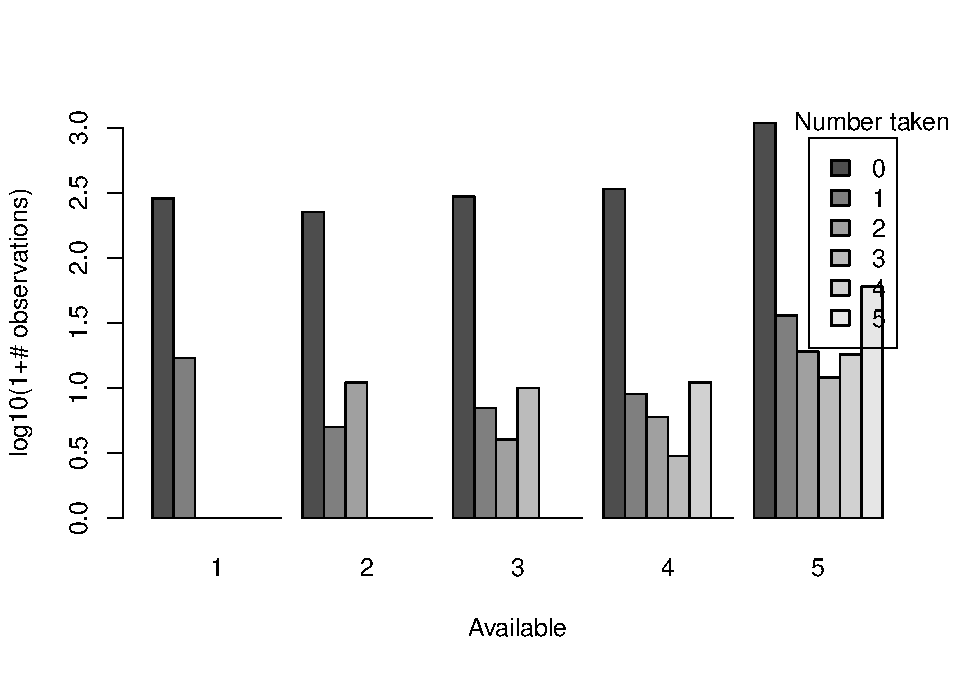
\includegraphics{Lab_2_modified_files/figure-latex/unnamed-chunk-39-1.pdf}
The argument \texttt{cex} controls the size of the points. As you see
the size of the bubbles are bit too large, so we need to adjust it. In
addition, we need to adjust the scaling of the axis.

\begin{Shaded}
\begin{Highlighting}[]
\KeywordTok{plot}\NormalTok{(}\StringTok{`}\DataTypeTok{Seeds taken}\StringTok{`} \OperatorTok{~}\StringTok{ `}\DataTypeTok{Seeds available}\StringTok{`}\NormalTok{,}\DataTypeTok{data=}\NormalTok{t2,}\DataTypeTok{cex=}\KeywordTok{log}\NormalTok{(val)}\OperatorTok{*}\DecValTok{2}\NormalTok{,}
        \DataTypeTok{xlim =} \KeywordTok{c}\NormalTok{(}\FloatTok{0.3}\NormalTok{,}\FloatTok{5.8}\NormalTok{),}\DataTypeTok{ylim=}\KeywordTok{c}\NormalTok{(}\OperatorTok{-}\FloatTok{0.5}\NormalTok{,}\FloatTok{5.5}\NormalTok{))}
\end{Highlighting}
\end{Shaded}

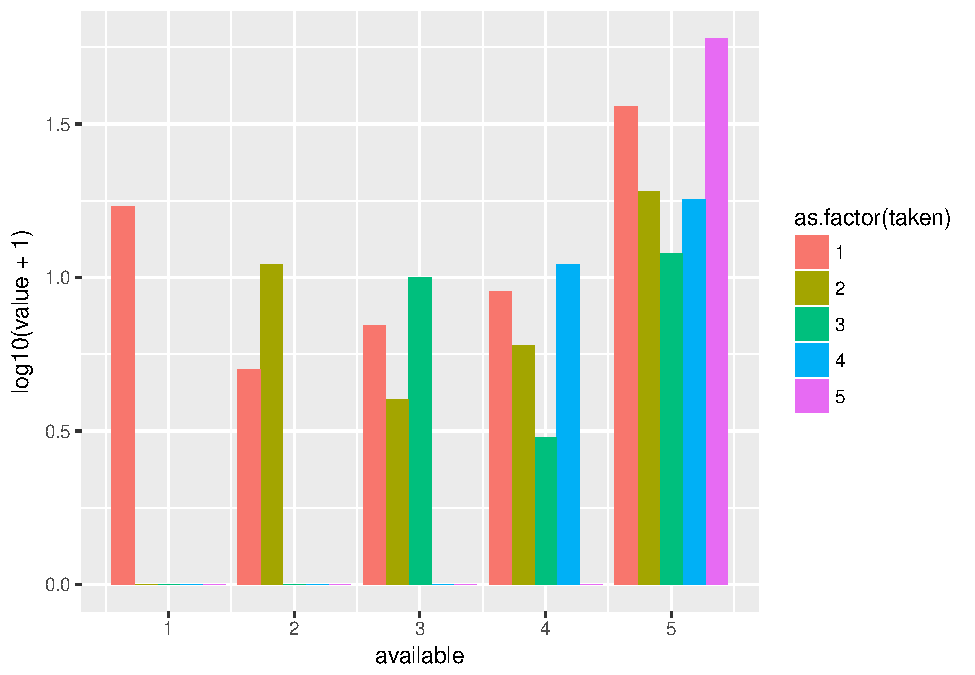
\includegraphics{Lab_2_modified_files/figure-latex/unnamed-chunk-40-1.pdf}

In ggplot this can be done as follows

\begin{Shaded}
\begin{Highlighting}[]
\KeywordTok{library}\NormalTok{(ggplot2)}
    \KeywordTok{ggplot}\NormalTok{(}\DataTypeTok{data=}\NormalTok{t2)}\OperatorTok{+}
\StringTok{        }\KeywordTok{geom_point}\NormalTok{(}\KeywordTok{aes}\NormalTok{(}\DataTypeTok{x =} \StringTok{`}\DataTypeTok{Seeds available}\StringTok{`}\NormalTok{, }\DataTypeTok{y =} \StringTok{`}\DataTypeTok{Seeds taken}\StringTok{`}\NormalTok{, }
                       \DataTypeTok{size =} \KeywordTok{log}\NormalTok{(val)}\OperatorTok{/}\DecValTok{2}\NormalTok{))}\OperatorTok{+}
\StringTok{      }\KeywordTok{ylab}\NormalTok{(}\StringTok{"Seeds taken"}\NormalTok{)}\OperatorTok{+}
\StringTok{      }\KeywordTok{xlab}\NormalTok{(}\StringTok{"Seeds available"}\NormalTok{)}
\end{Highlighting}
\end{Shaded}

\begin{verbatim}
## Warning in sqrt(x): NaNs produced
\end{verbatim}

\begin{verbatim}
## Warning: Removed 10 rows containing missing values (geom_point).
\end{verbatim}

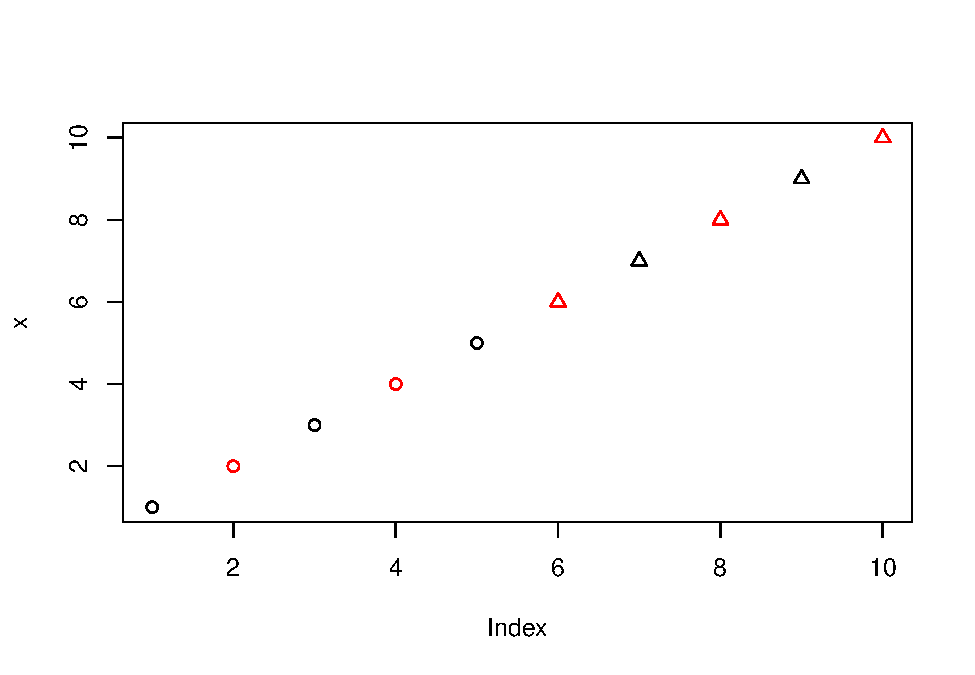
\includegraphics{Lab_2_modified_files/figure-latex/unnamed-chunk-41-1.pdf}

In \texttt{ggplot2} you need to specify the dataset the variables come
from. You do this throug \texttt{data=...}, a specification of type of
plot, a point plot can be specified through \texttt{geom\_point}, a
specifcation of the aesthetics (\texttt{aes(x...,y...)}) determines what
is plotted on the axes of the point plot. If data is specified in the
\texttt{ggplot} statement, it means that all plotting commands below
\texttt{ggplot(...)+} use that dataframe as reference. If the size
command is put inside the \texttt{aes} then size is dependent on some
variable, if put outside the \texttt{aes} it requires a single value
(similarly for e.g. \texttt{colour}, \texttt{linetype} and
\texttt{shape}). New commands can be added to the first statement
(\texttt{ggplot}) by adding a \texttt{+} after each line. If a column
name contains a space you can refer to it by putting it between
backticks: \texttt{...}

We could add the number of observations to the plot (\texttt{plot})
using the command \texttt{text}. The function \texttt{text} needs at
least three arguments, the x position and the y position of the text and
the text to be printed at this position. \texttt{text} allows vectors
for each of those arguments. Therefore we can write:

\begin{Shaded}
\begin{Highlighting}[]
\KeywordTok{plot}\NormalTok{(}\StringTok{`}\DataTypeTok{Seeds taken}\StringTok{`} \OperatorTok{~}\StringTok{ `}\DataTypeTok{Seeds available}\StringTok{`}\NormalTok{,}\DataTypeTok{data=}\NormalTok{t2,}\DataTypeTok{cex=}\KeywordTok{log}\NormalTok{(val)}\OperatorTok{*}\DecValTok{2}\NormalTok{,}
        \DataTypeTok{xlim =} \KeywordTok{c}\NormalTok{(}\FloatTok{0.3}\NormalTok{,}\FloatTok{5.8}\NormalTok{),}\DataTypeTok{ylim=}\KeywordTok{c}\NormalTok{(}\OperatorTok{-}\FloatTok{0.5}\NormalTok{,}\FloatTok{5.5}\NormalTok{))}
\KeywordTok{text}\NormalTok{(t2[,}\DecValTok{1}\NormalTok{],t2[,}\DecValTok{2}\NormalTok{],t2[,}\DecValTok{3}\NormalTok{])}
\end{Highlighting}
\end{Shaded}

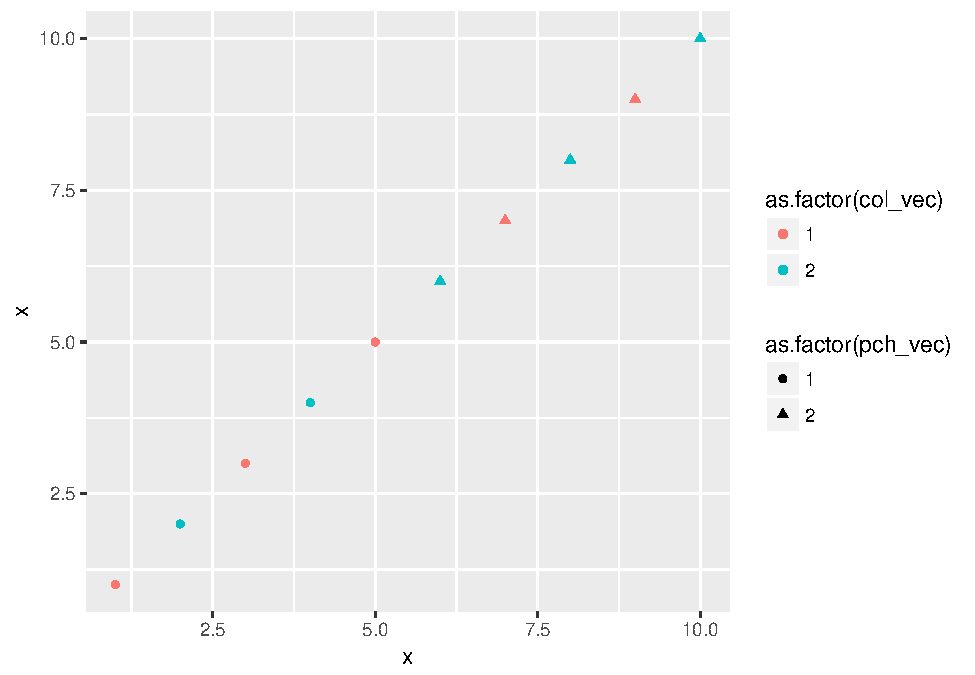
\includegraphics{Lab_2_modified_files/figure-latex/unnamed-chunk-42-1.pdf}

\textbf{Exercise 2.1} Change the size of the printed numbers and remove
the zeros from the graph.

\textbf{Exercise 2.2}: In general, you can specify plotting characters
and colors in parallel with your data, so that different points get
plotted with different plotting characters and colors. For example:

\begin{Shaded}
\begin{Highlighting}[]
\NormalTok{x =}\StringTok{ }\DecValTok{1}\OperatorTok{:}\DecValTok{10}
\NormalTok{col_vec =}\StringTok{ }\KeywordTok{rep}\NormalTok{(}\DecValTok{1}\OperatorTok{:}\DecValTok{2}\NormalTok{, }\DataTypeTok{length =} \DecValTok{10}\NormalTok{)}
\NormalTok{pch_vec =}\StringTok{ }\KeywordTok{rep}\NormalTok{(}\DecValTok{1}\OperatorTok{:}\DecValTok{2}\NormalTok{, }\DataTypeTok{each =} \DecValTok{5}\NormalTok{)}
\KeywordTok{plot}\NormalTok{(x, }\DataTypeTok{col =}\NormalTok{ col_vec, }\DataTypeTok{pch =}\NormalTok{ pch_vec)}
\end{Highlighting}
\end{Shaded}

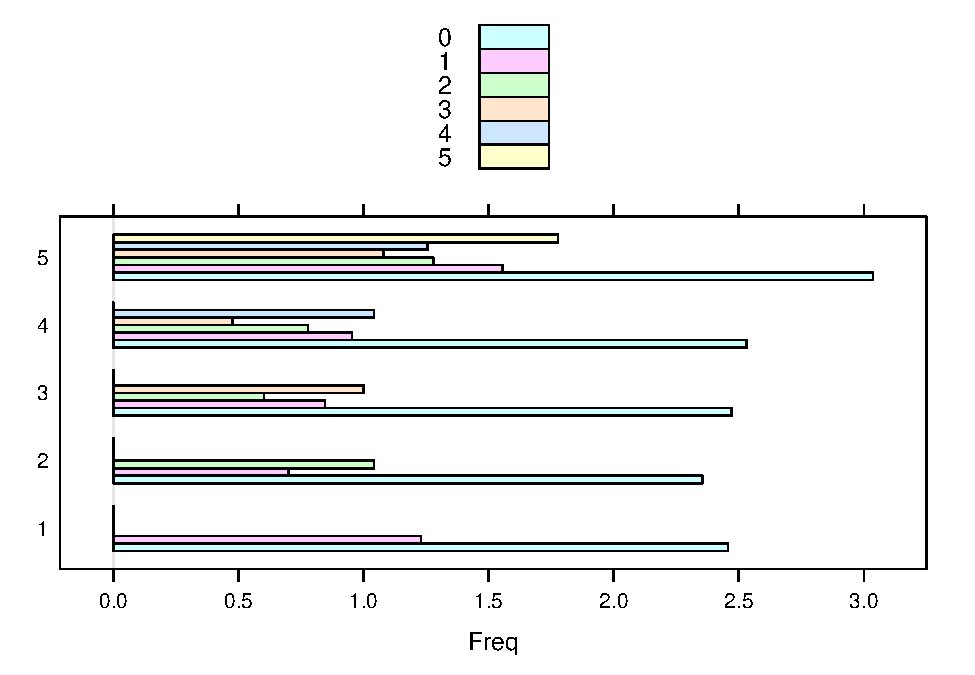
\includegraphics{Lab_2_modified_files/figure-latex/unnamed-chunk-43-1.pdf}
To use \texttt{col\_vec} and \texttt{pch\_vec} in \texttt{ggplot2} we
need to make them factors

\begin{Shaded}
\begin{Highlighting}[]
 \KeywordTok{ggplot}\NormalTok{()}\OperatorTok{+}
\StringTok{   }\KeywordTok{geom_point}\NormalTok{(}\KeywordTok{aes}\NormalTok{(}\DataTypeTok{x=}\NormalTok{x,}\DataTypeTok{y=}\NormalTok{x,}\DataTypeTok{shape=}\KeywordTok{as.factor}\NormalTok{(pch_vec),}\DataTypeTok{colour=}\KeywordTok{as.factor}\NormalTok{(col_vec)))}
\end{Highlighting}
\end{Shaded}

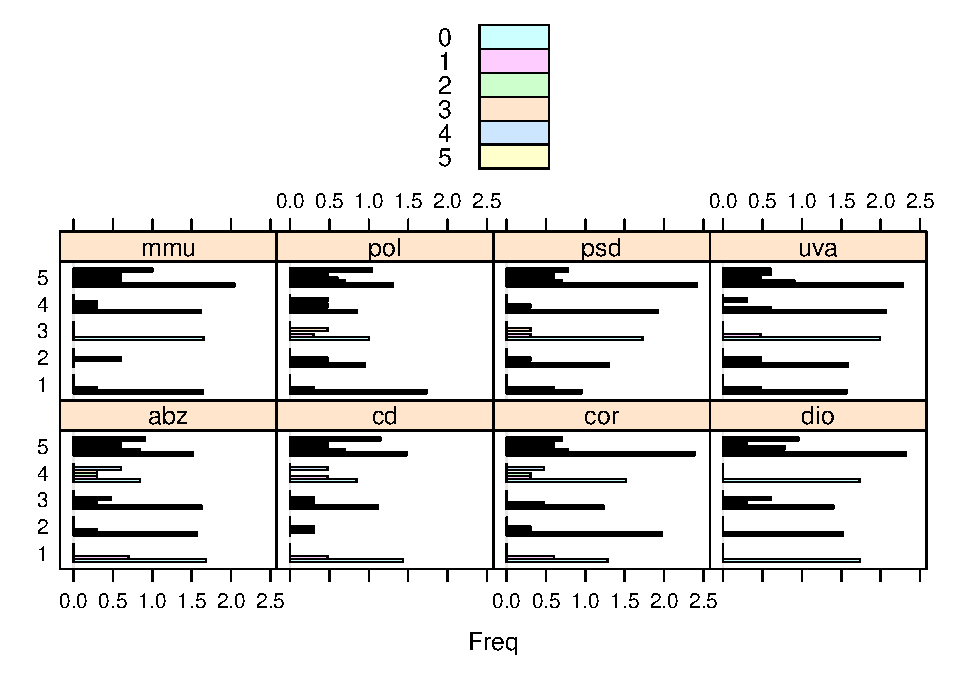
\includegraphics{Lab_2_modified_files/figure-latex/unnamed-chunk-44-1.pdf}

\subsection{2.1 Bar plot (with error
bars)}\label{bar-plot-with-error-bars}

The command to produce the barplot (Figure 3) was:

\begin{Shaded}
\begin{Highlighting}[]
\KeywordTok{barplot}\NormalTok{(}\KeywordTok{t}\NormalTok{(}\KeywordTok{log10}\NormalTok{(t1 }\OperatorTok{+}\StringTok{ }\DecValTok{1}\NormalTok{)), }\DataTypeTok{beside =} \OtherTok{TRUE}\NormalTok{, }\DataTypeTok{legend =} \OtherTok{TRUE}\NormalTok{, }\DataTypeTok{xlab =} \StringTok{"Available"}\NormalTok{,}
 \DataTypeTok{ylab =} \StringTok{"log10(1+# observations)"}\NormalTok{)}
\NormalTok{op =}\StringTok{ }\KeywordTok{par}\NormalTok{(}\DataTypeTok{xpd =} \OtherTok{TRUE}\NormalTok{)}
\KeywordTok{text}\NormalTok{(}\FloatTok{34.5}\NormalTok{, }\FloatTok{3.05}\NormalTok{, }\StringTok{"Number taken"}\NormalTok{)}
\end{Highlighting}
\end{Shaded}

\includegraphics{Lab_2_modified_files/figure-latex/unnamed-chunk-45-1.pdf}

\begin{Shaded}
\begin{Highlighting}[]
\KeywordTok{par}\NormalTok{(op)}
\end{Highlighting}
\end{Shaded}

Alternatively through \texttt{ggplot}

\begin{Shaded}
\begin{Highlighting}[]
\KeywordTok{ggplot}\NormalTok{(}\DataTypeTok{data=}\NormalTok{t2)}\OperatorTok{+}
\StringTok{  }\KeywordTok{geom_bar}\NormalTok{(}\KeywordTok{aes}\NormalTok{(}\DataTypeTok{x=}\StringTok{`}\DataTypeTok{Seeds available}\StringTok{`}\NormalTok{,}\DataTypeTok{y=}\KeywordTok{log10}\NormalTok{(val}\OperatorTok{+}\DecValTok{1}\NormalTok{),}
               \DataTypeTok{fill=}\KeywordTok{as.factor}\NormalTok{(}\StringTok{`}\DataTypeTok{Seeds taken}\StringTok{`}\NormalTok{)),}
           \DataTypeTok{stat=}\StringTok{"identity"}\NormalTok{,}\DataTypeTok{position=}\KeywordTok{position_dodge}\NormalTok{())}
\end{Highlighting}
\end{Shaded}

\includegraphics{Lab_2_modified_files/figure-latex/unnamed-chunk-46-1.pdf}
Again through \texttt{aes} we specify what is on the \texttt{x} and
\texttt{y}. Through \texttt{fill} we subdivide the bars by the values in
\texttt{taken}. \texttt{stat=identity} expresses that the values
assigned to \texttt{y} will be used (compare \texttt{stat="count"}).
Through specifying \texttt{position\_dodge()} bars are printed side by
side instead of stacked bars (\texttt{position\_fill()}).

More impressively, the ggplot package can automatically plot a barplot
of a three-way cross-tabulation (one barplot per species): try

\begin{Shaded}
\begin{Highlighting}[]
\NormalTok{t1.species =}\StringTok{ }\KeywordTok{table}\NormalTok{(data}\OperatorTok{$}\NormalTok{available,data}\OperatorTok{$}\NormalTok{remaining,data}\OperatorTok{$}\NormalTok{species)}
\NormalTok{t1.species =}\StringTok{ }\KeywordTok{melt}\NormalTok{(t1.species,}\DataTypeTok{varnames=}\KeywordTok{c}\NormalTok{(}\StringTok{"Seeds available"}\NormalTok{,}\StringTok{"Seeds taken"}\NormalTok{,}
                                        \StringTok{"species"}\NormalTok{),}\DataTypeTok{value.name=}\StringTok{"val"}\NormalTok{)}
\KeywordTok{ggplot}\NormalTok{(}\DataTypeTok{data=}\NormalTok{t1.species)}\OperatorTok{+}
\StringTok{  }\KeywordTok{geom_bar}\NormalTok{(}\KeywordTok{aes}\NormalTok{(}\DataTypeTok{x=}\StringTok{`}\DataTypeTok{Seeds available}\StringTok{`}\NormalTok{,}\DataTypeTok{y=}\KeywordTok{log10}\NormalTok{(val}\OperatorTok{+}\DecValTok{1}\NormalTok{),}
               \DataTypeTok{fill=}\KeywordTok{as.factor}\NormalTok{(}\StringTok{`}\DataTypeTok{Seeds taken}\StringTok{`}\NormalTok{)),}\DataTypeTok{stat=}\StringTok{"identity"}\NormalTok{,}
           \DataTypeTok{position=}\KeywordTok{position_dodge}\NormalTok{())}\OperatorTok{+}
\StringTok{  }\KeywordTok{facet_wrap}\NormalTok{(}\OperatorTok{~}\NormalTok{species)}\OperatorTok{+}
\StringTok{  }\KeywordTok{coord_flip}\NormalTok{()}
\end{Highlighting}
\end{Shaded}

\includegraphics{Lab_2_modified_files/figure-latex/unnamed-chunk-47-1.pdf}
with \texttt{facet\_wrap} a sequence of panels is made a specified by
the variable behind the \texttt{\textasciitilde{}}. The
\texttt{coord\_flip} rotates the plot.

\textbf{Exercise 2.2}: Restricting your analysis to only the
observations with 5 seeds available, create a barplot showing the
distribution of number of seeds taken broken down by species. Choose
whether you do this with \texttt{ggplot2} or through the base
\texttt{plot} function.

To add error bars to the barplot, one need to calculate the standard
error of the means. We want to plot the standard error on top of the
fraction seeds taken

First, compute the fraction taken:

\begin{Shaded}
\begin{Highlighting}[]
\NormalTok{data}\OperatorTok{$}\NormalTok{frac_taken =}\StringTok{ }\NormalTok{data}\OperatorTok{$}\NormalTok{taken}\OperatorTok{/}\NormalTok{data}\OperatorTok{$}\NormalTok{available}
\end{Highlighting}
\end{Shaded}

Computing the mean fraction taken for each number of seeds available,
using the \texttt{tapply()} function: \texttt{tapply()} (``table
apply'', pronounced ``t apply''), is an extension of the
\texttt{table()} function; it splits a specified vector into groups
according to the factors provided, then applies a function (e.g.
\texttt{mean()} or \texttt{sd()}) to each group. This idea of applying a
function to a set of objects is a very general, very powerful idea in
data manipulation with \texttt{R}; in due course we'll learn about
\texttt{apply()} (apply a function to rows and columns of matrices),
\texttt{lapply()} (apply a function to lists), \texttt{sapply()} (apply
a function to lists and simplify), and \texttt{mapply()} (apply a
function to multiple lists). For the present, though,

\begin{Shaded}
\begin{Highlighting}[]
\NormalTok{mean_frac_by_avail =}\StringTok{ }\KeywordTok{tapply}\NormalTok{(data}\OperatorTok{$}\NormalTok{frac_taken, data}\OperatorTok{$}\NormalTok{available, mean)}
\end{Highlighting}
\end{Shaded}

computes the mean of \texttt{frac\_taken} for each group defined by a
different value of available (R automatically converts available into a
factor temporarily for this purpose). If you want to compute the mean by
group for more than one variable in a data set, use
\texttt{aggregate()}. We can also calculate the standard errors,
\(\frac{\sigma}{\sqrt(n)}\):

\begin{Shaded}
\begin{Highlighting}[]
\NormalTok{n_by_avail =}\StringTok{ }\KeywordTok{table}\NormalTok{(data}\OperatorTok{$}\NormalTok{available)}
\NormalTok{se_by_avail =}\StringTok{ }\KeywordTok{tapply}\NormalTok{(data}\OperatorTok{$}\NormalTok{frac_taken, data}\OperatorTok{$}\NormalTok{available, sd)}\OperatorTok{/}
\StringTok{              }\KeywordTok{sqrt}\NormalTok{(n_by_avail)}
\end{Highlighting}
\end{Shaded}

First we plot a barplot after which we add arrows with an angle of 90
degrees. To position the error bars at the middle of the bars we need to
retrieve those positions from the barplot command. This can be done
through assigning a name \texttt{bara} to the barplot object and using
those positions as x coordinates.

\begin{Shaded}
\begin{Highlighting}[]
\NormalTok{bara =}\StringTok{ }\KeywordTok{barplot}\NormalTok{(mean_frac_by_avail,}\DataTypeTok{ylim=}\KeywordTok{c}\NormalTok{(}\DecValTok{0}\NormalTok{,}\FloatTok{0.09}\NormalTok{))}
\CommentTok{# hack: we draw arrows but with very special "arrowheads"}
\KeywordTok{arrows}\NormalTok{(bara[,}\DecValTok{1}\NormalTok{],mean_frac_by_avail}\OperatorTok{-}\NormalTok{se_by_avail,bara[,}\DecValTok{1}\NormalTok{], }
\NormalTok{       mean_frac_by_avail}\OperatorTok{+}\NormalTok{se_by_avail, }\DataTypeTok{length=}\FloatTok{0.05}\NormalTok{, }\DataTypeTok{angle=}\DecValTok{90}\NormalTok{, }\DataTypeTok{code=}\DecValTok{3}\NormalTok{)}
\end{Highlighting}
\end{Shaded}

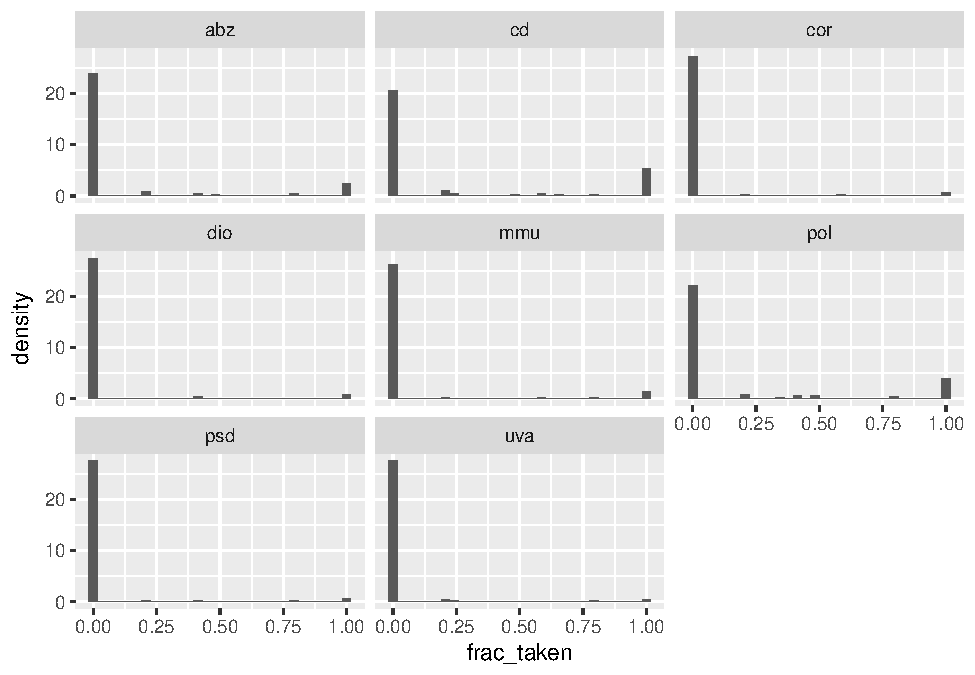
\includegraphics{Lab_2_modified_files/figure-latex/unnamed-chunk-52-1.pdf}

With \texttt{ggplot2} this is possible through the following syntax.
Note that there is a convenient function, called \texttt{summarySE} in
the \texttt{Rmisc} package to compute the means and se:

\begin{Shaded}
\begin{Highlighting}[]
\KeywordTok{library}\NormalTok{(Rmisc)}
\end{Highlighting}
\end{Shaded}

\begin{verbatim}
## Loading required package: lattice
\end{verbatim}

\begin{verbatim}
## Loading required package: plyr
\end{verbatim}

\begin{Shaded}
\begin{Highlighting}[]
\NormalTok{sum.data =}\StringTok{ }\KeywordTok{summarySE}\NormalTok{(data,}\DataTypeTok{measurevar=} \StringTok{"frac_taken"}\NormalTok{,}\DataTypeTok{groupvars=}\KeywordTok{c}\NormalTok{(}\StringTok{"available"}\NormalTok{))}
\NormalTok{pd =}\StringTok{ }\KeywordTok{position_dodge}\NormalTok{(}\DecValTok{0}\NormalTok{) }
\KeywordTok{ggplot}\NormalTok{(}\KeywordTok{aes}\NormalTok{(}\DataTypeTok{x=}\NormalTok{available,}\DataTypeTok{y=}\NormalTok{frac_taken),}\DataTypeTok{data=}\NormalTok{sum.data)}\OperatorTok{+}\StringTok{ }
\StringTok{  }\KeywordTok{geom_bar}\NormalTok{(,}\DataTypeTok{stat=}\StringTok{"identity"}\NormalTok{)}\OperatorTok{+}
\StringTok{  }\KeywordTok{geom_errorbar}\NormalTok{(}\KeywordTok{aes}\NormalTok{(}\DataTypeTok{ymin=}\NormalTok{frac_taken}\OperatorTok{-}\NormalTok{se, }\DataTypeTok{ymax=}\NormalTok{frac_taken}\OperatorTok{+}\NormalTok{se),}
                \DataTypeTok{stat=}\StringTok{"identity"}\NormalTok{, }\DataTypeTok{position=}\NormalTok{pd)}
\end{Highlighting}
\end{Shaded}

\includegraphics{Lab_2_modified_files/figure-latex/unnamed-chunk-53-1.pdf}
Make sure that the data reference is in the \texttt{ggplot()} function
so all other functions such as \texttt{geom\_bar} and
\texttt{geom\_errobar} make use of the same \texttt{data.frame}.

\section{2.4 Histogram by species}\label{histogram-by-species}

To make a histogram we can use the function \texttt{hist}:

\begin{Shaded}
\begin{Highlighting}[]
\KeywordTok{hist}\NormalTok{(data}\OperatorTok{$}\NormalTok{frac_taken)}
\end{Highlighting}
\end{Shaded}

\includegraphics{Lab_2_modified_files/figure-latex/unnamed-chunk-54-1.pdf}
To draw a histogram per species, we need to split the data into a list
with each element representing a species.

\begin{Shaded}
\begin{Highlighting}[]
\NormalTok{data.s =}\StringTok{ }\KeywordTok{split}\NormalTok{(data}\OperatorTok{$}\NormalTok{frac_taken,}\KeywordTok{list}\NormalTok{(data}\OperatorTok{$}\NormalTok{species))}
\end{Highlighting}
\end{Shaded}

Next, we use \texttt{sapply} to plot the histograms.

\begin{Shaded}
\begin{Highlighting}[]
\KeywordTok{par}\NormalTok{(}\DataTypeTok{mfrow=}\KeywordTok{c}\NormalTok{(}\DecValTok{4}\NormalTok{,}\DecValTok{2}\NormalTok{),}\DataTypeTok{oma=}\KeywordTok{c}\NormalTok{(}\DecValTok{0}\NormalTok{,}\DecValTok{0}\NormalTok{,}\DecValTok{0}\NormalTok{,}\DecValTok{0}\NormalTok{),}\DataTypeTok{mar=}\KeywordTok{c}\NormalTok{(}\DecValTok{4}\NormalTok{,}\DecValTok{4}\NormalTok{,}\FloatTok{0.1}\NormalTok{,}\FloatTok{0.1}\NormalTok{))}
\KeywordTok{sapply}\NormalTok{(data.s,hist,}\DataTypeTok{main=}\StringTok{""}\NormalTok{)}
\CommentTok{# or equivalently}
\ControlFlowTok{for}\NormalTok{ (i }\ControlFlowTok{in} \DecValTok{1}\OperatorTok{:}\DecValTok{8}\NormalTok{)\{}
  \KeywordTok{hist}\NormalTok{(data.s[[i]],}\DataTypeTok{main=}\StringTok{""}\NormalTok{)}
\NormalTok{\}}
\end{Highlighting}
\end{Shaded}

With \texttt{ggplot2} you can get the frequencies less easily, so will
be plot the counts

\begin{Shaded}
\begin{Highlighting}[]
\KeywordTok{ggplot}\NormalTok{(}\DataTypeTok{data=}\NormalTok{data)}\OperatorTok{+}
\KeywordTok{geom_bar}\NormalTok{(}\KeywordTok{aes}\NormalTok{(}\DataTypeTok{x=}\NormalTok{frac_taken),}\DataTypeTok{stat=}\StringTok{"count"}\NormalTok{)}\OperatorTok{+}
\StringTok{  }\KeywordTok{facet_wrap}\NormalTok{(}\OperatorTok{~}\StringTok{ }\NormalTok{species)}
\end{Highlighting}
\end{Shaded}

\includegraphics{Lab_2_modified_files/figure-latex/unnamed-chunk-57-1.pdf}

\begin{Shaded}
\begin{Highlighting}[]
\KeywordTok{ggplot}\NormalTok{(}\DataTypeTok{data=}\NormalTok{data,}\KeywordTok{aes}\NormalTok{(}\DataTypeTok{x=}\NormalTok{frac_taken))}\OperatorTok{+}
\StringTok{  }\KeywordTok{geom_histogram}\NormalTok{(}\KeywordTok{aes}\NormalTok{(}\DataTypeTok{y =}\NormalTok{ ..density..))}\OperatorTok{+}
\StringTok{  }\KeywordTok{facet_wrap}\NormalTok{(}\OperatorTok{~}\NormalTok{species)}
\end{Highlighting}
\end{Shaded}

\begin{verbatim}
## `stat_bin()` using `bins = 30`. Pick better value with `binwidth`.
\end{verbatim}

\includegraphics{Lab_2_modified_files/figure-latex/unnamed-chunk-58-1.pdf}

\section{3. Measles Data}\label{measles-data}

I'm going to clear the workspace (\texttt{rm(list=ls()}) lists all the
objects in the workspace with \texttt{ls()} and then uses \texttt{rm()}
to remove them. It is recommend to have this code at the top of your
script, so every time you start working on the script you are sure the
memory is cleared. You can also Clear workspace from the menu (in
Rstudio the little brush in the topright panel)) and read in the measles
data, which are space separated and have a header:

\begin{Shaded}
\begin{Highlighting}[]
\KeywordTok{rm}\NormalTok{(}\DataTypeTok{list =} \KeywordTok{ls}\NormalTok{())}
\NormalTok{data =}\StringTok{ }\KeywordTok{read.table}\NormalTok{(}\StringTok{"ewcitmeas.dat"}\NormalTok{, }\DataTypeTok{header =} \OtherTok{TRUE}\NormalTok{, }\DataTypeTok{na.strings =} \StringTok{"*"}\NormalTok{)}
\end{Highlighting}
\end{Shaded}

\texttt{year}, \texttt{mon}, and \texttt{day} were read in as integers:
I'll create a date variable as described above. For convenience, I'm
also defining a variable with the city names.

\begin{Shaded}
\begin{Highlighting}[]
\NormalTok{date =}\StringTok{ }\KeywordTok{as.Date}\NormalTok{(}\KeywordTok{paste}\NormalTok{(data}\OperatorTok{$}\NormalTok{year }\OperatorTok{+}\StringTok{ }\DecValTok{1900}\NormalTok{, data}\OperatorTok{$}\NormalTok{mon, data}\OperatorTok{$}\NormalTok{day, }\DataTypeTok{sep =} \StringTok{"/"}\NormalTok{))}
\NormalTok{city_names =}\StringTok{ }\KeywordTok{colnames}\NormalTok{(data)[}\DecValTok{4}\OperatorTok{:}\DecValTok{10}\NormalTok{]}
\end{Highlighting}
\end{Shaded}

Later on it will be useful to have the data in long format. It's easiest
to do use \texttt{melt} for this purpose. Note that only need to select
the appropriate columns to melt (i.e.~4-11).

\begin{Shaded}
\begin{Highlighting}[]
\KeywordTok{library}\NormalTok{(reshape2)}
\NormalTok{data=}\StringTok{ }\KeywordTok{cbind}\NormalTok{(data,date)}
\NormalTok{data_long =}\StringTok{ }\KeywordTok{melt}\NormalTok{(data[,}\DecValTok{4}\OperatorTok{:}\DecValTok{11}\NormalTok{],}\DataTypeTok{id.vars=}\DecValTok{8}\NormalTok{,}\DataTypeTok{variable.name =} \StringTok{"city"}\NormalTok{,}\DataTypeTok{value.name=}\StringTok{"incidence"}\NormalTok{)}
\end{Highlighting}
\end{Shaded}

\subsection{3.1 Multiple-line plots}\label{multiple-line-plots}

We can make a plot with multiple lines as follows. We first setup the
plotting region using \texttt{plot} followed by the function
\texttt{lines} to add lines to the existing plot. Note that in the
plotting command \texttt{type="l"} is used to specify that lines are
drawn instead of point (\texttt{type="p}, the default). A legend can be
added by adding the function \texttt{legend}

\begin{Shaded}
\begin{Highlighting}[]
\NormalTok{data_long.s =}\StringTok{ }\KeywordTok{split}\NormalTok{(data_long,data_long}\OperatorTok{$}\NormalTok{city)}
\KeywordTok{plot}\NormalTok{(incidence }\OperatorTok{~}\StringTok{ }\NormalTok{date,}\DataTypeTok{col=}\DecValTok{1}\NormalTok{,}\DataTypeTok{type=}\StringTok{"l"}\NormalTok{,}\DataTypeTok{data=}\NormalTok{data_long[data_long}\OperatorTok{$}\NormalTok{city }\OperatorTok{==}\StringTok{ "London"}\NormalTok{,])}
\NormalTok{unique.city =}\StringTok{ }\KeywordTok{unique}\NormalTok{(data_long}\OperatorTok{$}\NormalTok{city)}
\ControlFlowTok{for}\NormalTok{ (i }\ControlFlowTok{in} \DecValTok{2}\OperatorTok{:}\KeywordTok{length}\NormalTok{(unique.city))\{}
  \KeywordTok{lines}\NormalTok{(incidence }\OperatorTok{~}\StringTok{ }\NormalTok{date,}\DataTypeTok{type=}\StringTok{"l"}\NormalTok{,}
        \DataTypeTok{data=}\NormalTok{data_long[data_long}\OperatorTok{$}\NormalTok{city }\OperatorTok{==}\StringTok{ }\NormalTok{unique.city[i],],}\DataTypeTok{col=}\NormalTok{i)}
\NormalTok{\}}
\KeywordTok{legend}\NormalTok{(}\StringTok{"topright"}\NormalTok{,}\DataTypeTok{legend=}\NormalTok{unique.city,}\DataTypeTok{col=}\DecValTok{1}\OperatorTok{:}\DecValTok{8}\NormalTok{,}\DataTypeTok{lty=}\DecValTok{1}\NormalTok{)}
\end{Highlighting}
\end{Shaded}

With ggplot2 we specify

\begin{Shaded}
\begin{Highlighting}[]
\KeywordTok{ggplot}\NormalTok{() }\OperatorTok{+}
\StringTok{  }\KeywordTok{geom_line}\NormalTok{(}\KeywordTok{aes}\NormalTok{(}\DataTypeTok{x=}\NormalTok{date,}\DataTypeTok{y=}\NormalTok{incidence, }\DataTypeTok{colour=}\NormalTok{city),}\DataTypeTok{data=}\NormalTok{data_long)}
\end{Highlighting}
\end{Shaded}

\section{3.2 Histogram and density
plots}\label{histogram-and-density-plots}

I'll start by just collapsing all the incidence data into a single,
logged, non-NA vector (in this case I have to use
\texttt{c(as.matrix(x))} to collapse the data and remove all of the data
frame information):

\begin{Shaded}
\begin{Highlighting}[]
\NormalTok{allvals =}\StringTok{ }\KeywordTok{na.omit}\NormalTok{(}\KeywordTok{c}\NormalTok{(}\KeywordTok{as.matrix}\NormalTok{(data[, }\DecValTok{4}\OperatorTok{:}\DecValTok{10}\NormalTok{])))}
\NormalTok{logvals =}\StringTok{ }\KeywordTok{log10}\NormalTok{(}\DecValTok{1} \OperatorTok{+}\StringTok{ }\NormalTok{allvals)}
\end{Highlighting}
\end{Shaded}

The histogram (\texttt{hist()} command is fairly easy: the only tricks
are to leave room for the other lines that will go on the plot by
setting the y limits with ylim, and to specify that we want the data
plotted as relative frequencies, not numbers of counts
(\texttt{freq=FALSE} or \texttt{prob=TRUE}). This option tells
\texttt{R} to divide by total number of counts and then by the bin
width, so that the area covered by all the bars adds up to 1; this
scaling makes the vertical scale of the histogram compatible with a
density plot, or among different histograms with different number of
counts or bin widths (?? include in chapter ??).

\begin{Shaded}
\begin{Highlighting}[]
\KeywordTok{hist}\NormalTok{(logvals, }\DataTypeTok{col =} \StringTok{"gray"}\NormalTok{, }\DataTypeTok{main =} \StringTok{""}\NormalTok{, }\DataTypeTok{xlab =} \StringTok{"Log weekly incidence"}\NormalTok{,}
 \DataTypeTok{ylab =} \StringTok{"Density"}\NormalTok{, }\DataTypeTok{freq =} \OtherTok{FALSE}\NormalTok{, }\DataTypeTok{ylim =} \KeywordTok{c}\NormalTok{(}\DecValTok{0}\NormalTok{, }\FloatTok{0.6}\NormalTok{))}
\end{Highlighting}
\end{Shaded}

\includegraphics{Lab_2_modified_files/figure-latex/unnamed-chunk-65-1.pdf}
Adding lines for the density is straightforward, since R knows what to
do with a density object - in general, the lines command just adds lines
to a plot.

\begin{Shaded}
\begin{Highlighting}[]
\KeywordTok{lines}\NormalTok{(}\KeywordTok{density}\NormalTok{(logvals), }\DataTypeTok{lwd =} \DecValTok{2}\NormalTok{)}
\KeywordTok{lines}\NormalTok{(}\KeywordTok{density}\NormalTok{(logvals, }\DataTypeTok{adjust =} \FloatTok{0.5}\NormalTok{), }\DataTypeTok{lwd =} \DecValTok{2}\NormalTok{, }\DataTypeTok{lty =} \DecValTok{2}\NormalTok{)}
\end{Highlighting}
\end{Shaded}

With ggplot2 we specify:

\begin{Shaded}
\begin{Highlighting}[]
\KeywordTok{ggplot}\NormalTok{()}\OperatorTok{+}
\StringTok{  }\KeywordTok{geom_histogram}\NormalTok{(}\KeywordTok{aes}\NormalTok{(}\DataTypeTok{x=}\NormalTok{logvals,}\DataTypeTok{y=}\NormalTok{..density..))}\OperatorTok{+}
\StringTok{  }\KeywordTok{geom_density}\NormalTok{(}\KeywordTok{aes}\NormalTok{(}\DataTypeTok{x=}\NormalTok{logvals,}\DataTypeTok{y=}\NormalTok{..density..))}
\end{Highlighting}
\end{Shaded}

\begin{verbatim}
## `stat_bin()` using `bins = 30`. Pick better value with `binwidth`.
\end{verbatim}

\includegraphics{Lab_2_modified_files/figure-latex/unnamed-chunk-67-1.pdf}

\section{3.3 Scaling data}\label{scaling-data}

Scaling the incidence in each city by the population size, or by the
mean or maximum incidence in that city, begins to get us into some
non-trivial data manipulation. This process may actually be easier in
the wide format. Several useful commands: * \texttt{rowMeans()},
\texttt{rowSums()}, \texttt{colMeans()}, and \texttt{colSums()} will
compute the means or sums of columns efficiently. In this case we would
do something like \texttt{colMeans(data{[},4:10{]}}) to get the mean
incidence for each city.

\begin{itemize}
\item
  \texttt{apply()} is the more general command for running some command
  on each of a set of rows or columns. When you look at the help for
  apply() you'll see an argument called MARGIN, which specifies whether
  you want to operate on rows (1) or columns (2). For example,
  apply(data{[},4:10{]},1,mean) is the equivalent of
  rowMeans(data{[},4:10{]}), but we can also easily say (e.g.)
  apply(data{[},4:10{]},1,max) to get the maxima instead. Later, when
  you've gotten practice defining your own functions, you can apply any
  function - not just R's built-in functions.
\item
  \texttt{scale()} is a function for subtracting and dividing specified
  amounts out of the columns of a matrix. It is fairly flexible:
  scale(x,center=TRUE,scale=TRUE) will center by subtracting the means
  and then scale by dividing by the standard errors of the columns.
  Fairly obviously, setting either to FALSE will turn off that part of
  the operation. You can also specify a vector for either center or
  scale, in which case scale() will subtract or divide the columns by
  those vectors instead.
\end{itemize}

\textbf{Exercise 3.1}: figure out how to use apply() and scale() to
scale all columns so they have a minimum of 0 and a maximum of 1 (hint:
subtract the minimum and divide by (max-min)).

\section{3.4 Box-and-whisker and violin
plots}\label{box-and-whisker-and-violin-plots}

By this time, box-and-whisker and violin plots will (I hope) seem easy.
Since the labels get a little crowded (\texttt{R} is not really
sophisticated about dealing with axis labels-crowded labels), I'll use
the \texttt{substr()} (substring) command to abbreviate each city's name
to its first three letters.

\begin{Shaded}
\begin{Highlighting}[]
\NormalTok{city_abbr =}\StringTok{ }\KeywordTok{substr}\NormalTok{(city_names, }\DecValTok{1}\NormalTok{, }\DecValTok{3}\NormalTok{)}
\end{Highlighting}
\end{Shaded}

The \texttt{boxplot()} command uses a formula - the variable before the
\textasciitilde{} is the data and the variable after it is the factor to
use to split the data up.

\begin{Shaded}
\begin{Highlighting}[]
\KeywordTok{boxplot}\NormalTok{(}\KeywordTok{log10}\NormalTok{(}\DecValTok{1} \OperatorTok{+}\StringTok{ }\NormalTok{incidence) }\OperatorTok{~}\StringTok{ }\NormalTok{city, }\DataTypeTok{data =}\NormalTok{ data_long, }\DataTypeTok{ylab =} \StringTok{"Log(incidence+1)"}\NormalTok{,}
 \DataTypeTok{names =}\NormalTok{ city_abbr)}
\end{Highlighting}
\end{Shaded}

Or through ggplot

\begin{Shaded}
\begin{Highlighting}[]
\KeywordTok{ggplot}\NormalTok{(}\DataTypeTok{data=}\NormalTok{data_long)}\OperatorTok{+}
\StringTok{  }\KeywordTok{geom_boxplot}\NormalTok{((}\KeywordTok{aes}\NormalTok{(}\DataTypeTok{x=}\NormalTok{city,}\DataTypeTok{y=}\KeywordTok{log10}\NormalTok{(incidence}\OperatorTok{+}\DecValTok{1}\NormalTok{))))}
\end{Highlighting}
\end{Shaded}

If I want to make a violin plot, you can specify:

\begin{Shaded}
\begin{Highlighting}[]
\KeywordTok{ggplot}\NormalTok{(}\DataTypeTok{data=}\NormalTok{data_long)}\OperatorTok{+}
\StringTok{  }\KeywordTok{geom_violin}\NormalTok{((}\KeywordTok{aes}\NormalTok{(}\DataTypeTok{x=}\NormalTok{city,}\DataTypeTok{y=}\KeywordTok{log10}\NormalTok{(incidence}\OperatorTok{+}\DecValTok{1}\NormalTok{))))}
\end{Highlighting}
\end{Shaded}

\section{4. Continuous data}\label{continuous-data}

First let's make sure the earthquake data are accessible:

\begin{Shaded}
\begin{Highlighting}[]
\KeywordTok{data}\NormalTok{(quakes)}
\end{Highlighting}
\end{Shaded}

Luckily, most of the plots I drew in this section are fairly automatic.
To draw a scatterplot matrix, just use \texttt{pairs()} (base):

\begin{Shaded}
\begin{Highlighting}[]
\KeywordTok{pairs}\NormalTok{(quakes, }\DataTypeTok{pch =} \StringTok{"."}\NormalTok{)}
\end{Highlighting}
\end{Shaded}

\includegraphics{Lab_2_modified_files/figure-latex/unnamed-chunk-74-1.pdf}
(\texttt{pch="."} marks the data with a single-pixel point, which is
handy if you are fortunate enough to have a really big data set).

\textbf{Exercise 4.1}*: generate three new plots based on one of the
data sets in this lab, or on your own data.


\end{document}
